% Appendix Template

\newcommand{\major}{2}
\newcommand{\minor}{4}

\newcommand{\undPrefix}{\major_\minor}
\newcommand{\dotPrefix}{\major.\minor}
\newcommand{\scoPrefix}{\major-\minor}
\newcommand{\filePrefix}{\undPrefix/rff}

\chapter{Results of experiment \dotPrefix} % Main appendix title


\label{Appendix\scoPrefix} % Change X to a consecutive letter; for referencing this appendix elsewhere, use \ref{AppendixX}

These experiments are discussed \hyperref[disc:h2]{here}


%%%%%%%%%%%%%%%%%%%%%%%%%%%%%%%%%%%%%%%%%%%%%%
%%%%%%%%%%%%%%%%%%%%%%%%%%%%%%%%%%%%%%%%%%%%%%
%%%%%%%%%%%%%%%%%%%%%%%%%%%%%%%%%%%%%%%%%%%%%%
%% Empieza lo nuevo
%%%%%%%%%%%%%%%%%%%%%%%%%%%%%%%%%%%%%%%%%%%%%%
%%%%%%%%%%%%%%%%%%%%%%%%%%%%%%%%%%%%%%%%%%%%%%
%%%%%%%%%%%%%%%%%%%%%%%%%%%%%%%%%%%%%%%%%%%%%%

\begin{figure}[H]
  \centering
  \renewcommand{\filePrefix}{\undPrefix/rff}
  \begin{subfigure}[t]{0.5\linewidth}
    \centering\captionsetup{width=.8\linewidth}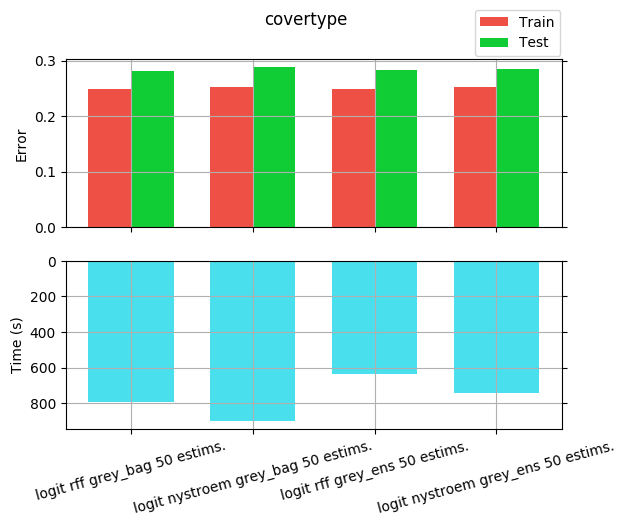
\includegraphics[width=\imgscale\linewidth]{Figures/\filePrefix/covertype}
    \caption{Exp 2.4 with Random Fourier Feautures with Covertype. Error is decreased by 15\% approx.}
    \label{fig:\undPrefix_covertype}
  \end{subfigure}%
  \renewcommand{\filePrefix}{\undPrefix/nys}%
  \begin{subfigure}[t]{0.5\linewidth}
    \centering\captionsetup{width=.8\linewidth}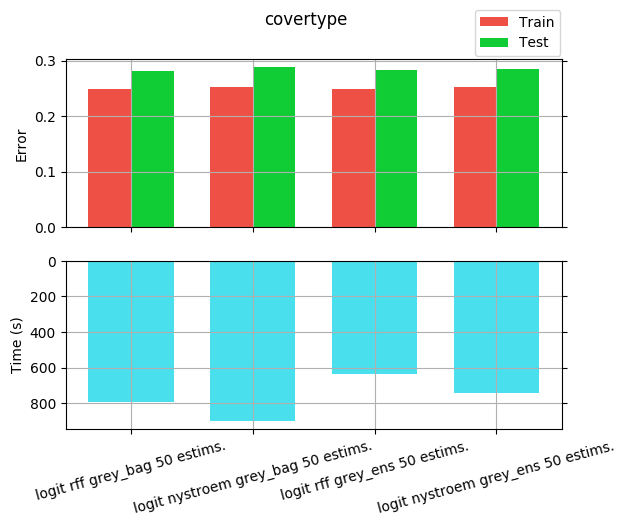
\includegraphics[width=\imgscale\linewidth]{Figures/\filePrefix/covertype}
    \caption{Exp 2.4 with \Nys\ with Covertype. Error is decreased by 15\% approx.}
    \label{fig:\undPrefix_covertype}
  \end{subfigure}%
\end{figure}


\begin{figure}[H]
  \centering
  \renewcommand{\filePrefix}{\undPrefix/rff}
  \begin{subfigure}[t]{0.5\linewidth}
    \centering\captionsetup{width=.8\linewidth}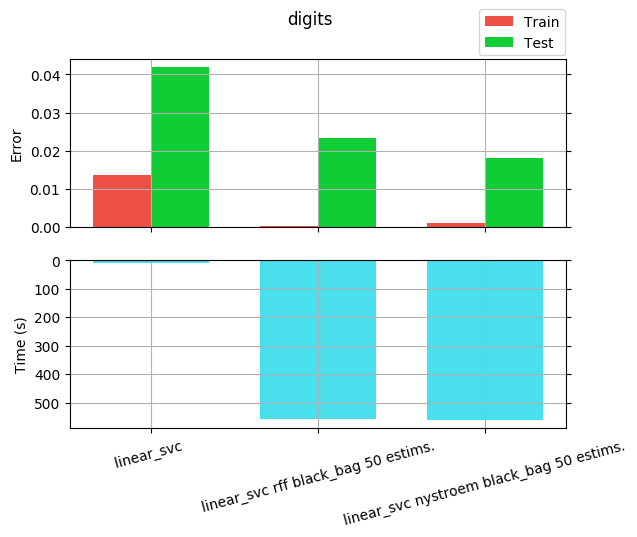
\includegraphics[width=\imgscale\linewidth]{Figures/\filePrefix/digits}
    \caption{Exp 2.4 with Random Fourier Feautures with Digits. Error is decreased by 2\% approx.}
    \label{fig:\undPrefix_digits}
  \end{subfigure}%
  \renewcommand{\filePrefix}{\undPrefix/nys}%
  \begin{subfigure}[t]{0.5\linewidth}
    \centering\captionsetup{width=.8\linewidth}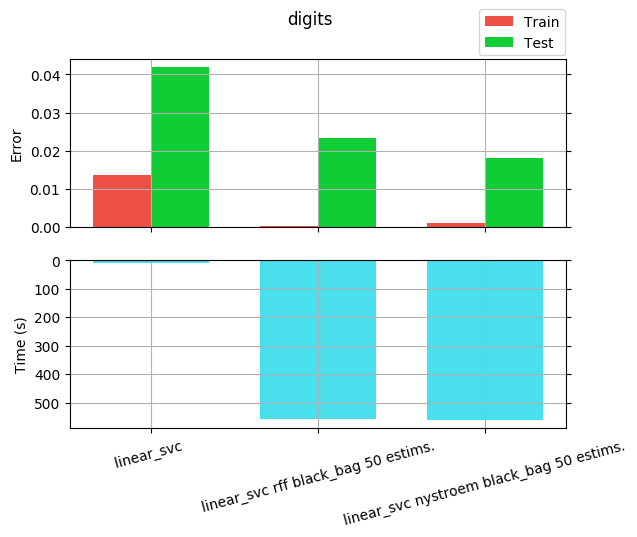
\includegraphics[width=\imgscale\linewidth]{Figures/\filePrefix/digits}
    \caption{Exp 2.4 with \Nys\ with Digits. Error is decreased by 2\% approx.}
    \label{fig:\undPrefix_digits}
  \end{subfigure}
\end{figure}


\begin{figure}[H]
  \centering
  \renewcommand{\filePrefix}{\undPrefix/rff}
  \begin{subfigure}[t]{0.5\linewidth}
    \centering\captionsetup{width=.8\linewidth}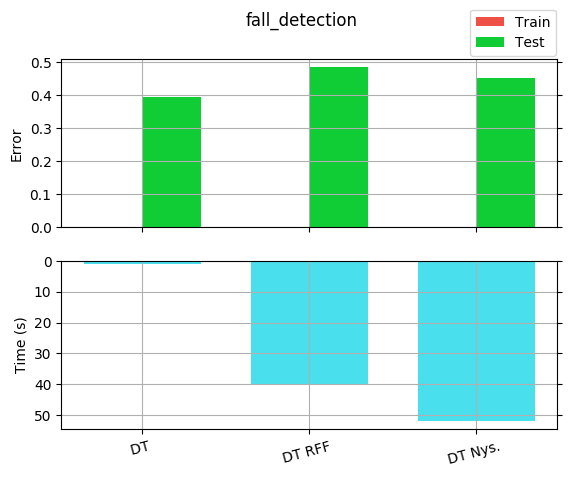
\includegraphics[width=\imgscale\linewidth]{Figures/\filePrefix/fall_detection}
    \caption{Exp 2.4 with Random Fourier Feautures with Fall Detection. Error is decreased by 2\% approx.}
    \label{fig:\undPrefix_fall_detection}
  \end{subfigure}%
  \renewcommand{\filePrefix}{\undPrefix/nys}%
  \begin{subfigure}[t]{0.5\linewidth}
    \centering\captionsetup{width=.8\linewidth}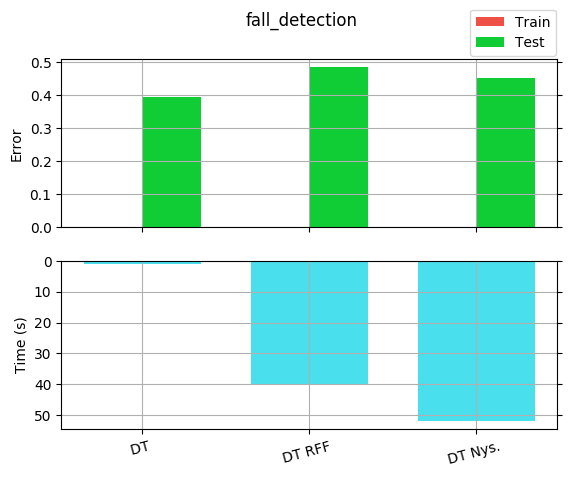
\includegraphics[width=\imgscale\linewidth]{Figures/\filePrefix/fall_detection}
    \caption{Exp 2.4 with \Nys\ with Fall Detection. Error is decreased by 2\% approx.}
    \label{fig:\undPrefix_fall_detection}
  \end{subfigure}%
\end{figure}


\begin{figure}[H]
  \centering
  \renewcommand{\filePrefix}{\undPrefix/rff}
  \begin{subfigure}[t]{0.5\linewidth}
    \centering\captionsetup{width=.8\linewidth}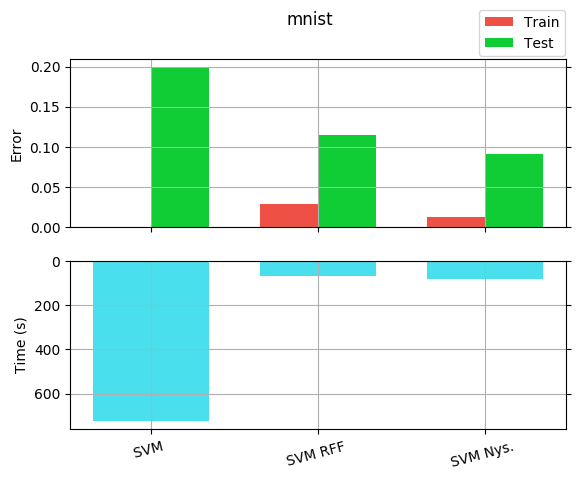
\includegraphics[width=\imgscale\linewidth]{Figures/\filePrefix/mnist}
    \caption{Exp 2.4 with Random Fourier Feautures with MNIST. Error is decreased by 10\% approx.}
    \label{fig:\undPrefix_mnist}
  \end{subfigure}%
  \renewcommand{\filePrefix}{\undPrefix/nys}%
  \begin{subfigure}[t]{0.5\linewidth}
    \centering\captionsetup{width=.8\linewidth}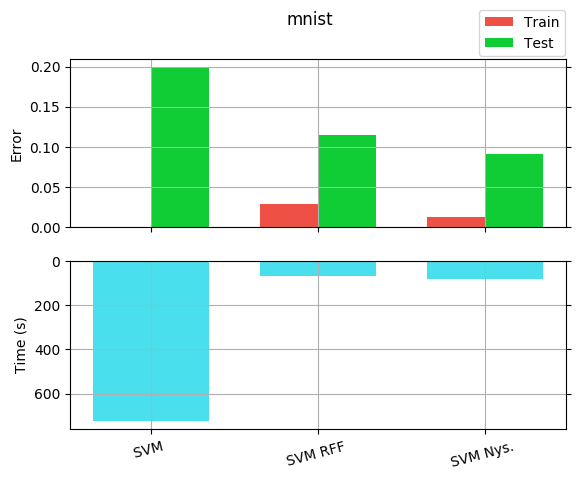
\includegraphics[width=\imgscale\linewidth]{Figures/\filePrefix/mnist}
    \caption{Exp 2.4 with \Nys\ with MNIST. Error is decreased by 10\% approx.}
    \label{fig:\undPrefix_mnist}
  \end{subfigure}
\end{figure}


\begin{figure}[H]
  \centering
  \renewcommand{\filePrefix}{\undPrefix/rff}
  \begin{subfigure}[t]{0.5\linewidth}
    \centering\captionsetup{width=.8\linewidth}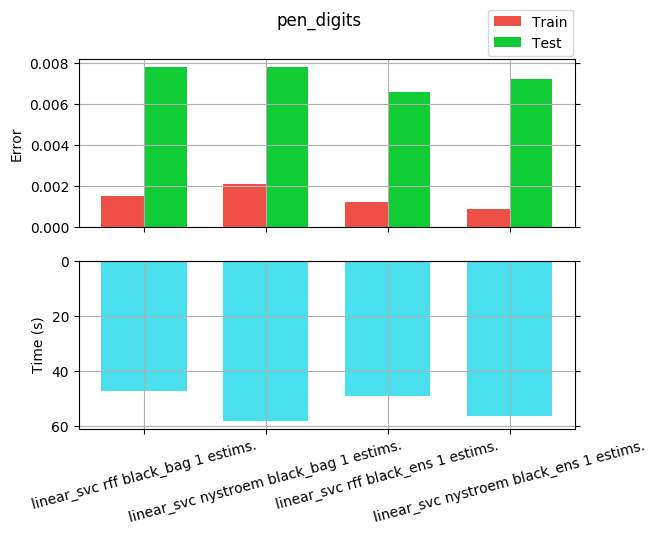
\includegraphics[width=\imgscale\linewidth]{Figures/\filePrefix/pen_digits}
    \caption{Exp 2.4 with Random Fourier Feautures with Pen Digits. Error is decreased by 5\% approx.}
    \label{fig:\undPrefix_pen_digits}
  \end{subfigure}%
  \renewcommand{\filePrefix}{\undPrefix/nys}%
  \begin{subfigure}[t]{0.5\linewidth}
    \centering\captionsetup{width=.8\linewidth}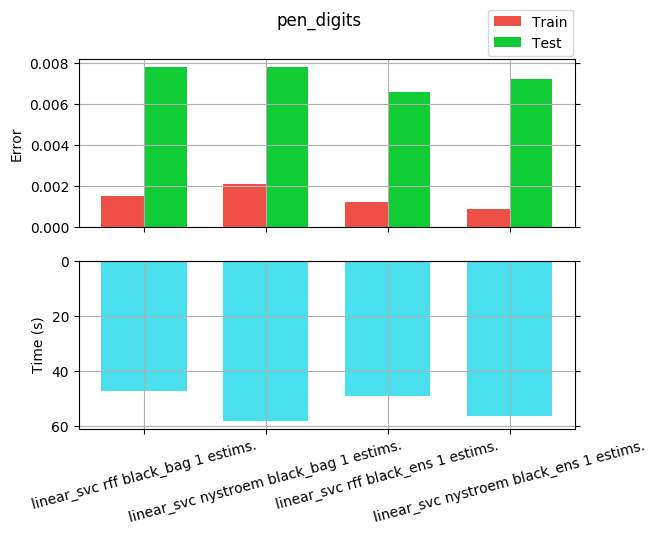
\includegraphics[width=\imgscale\linewidth]{Figures/\filePrefix/pen_digits}
    \caption{Exp 2.4 with \Nys\ with Pen Digits. Error is decreased by 5\% approx.}
    \label{fig:\undPrefix_pen_digits}
  \end{subfigure}%
\end{figure}


\begin{figure}[H]
  \centering
  \renewcommand{\filePrefix}{\undPrefix/rff}
  \begin{subfigure}[t]{0.5\linewidth}
    \centering\captionsetup{width=.8\linewidth}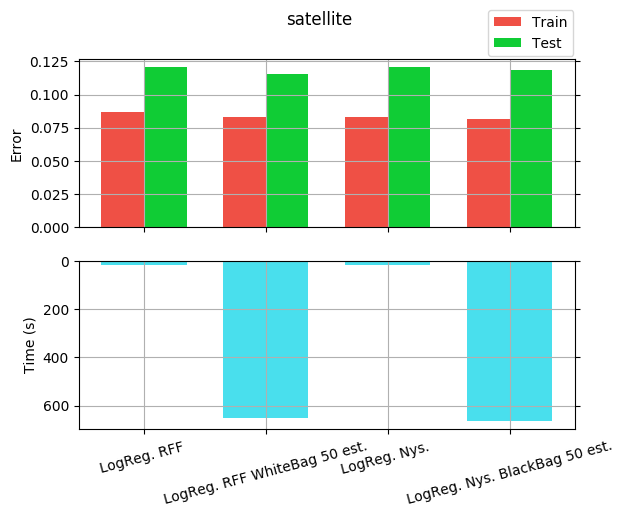
\includegraphics[width=\imgscale\linewidth]{Figures/\filePrefix/satellite}
    \caption{Exp 2.4 with Random Fourier Feautures with Satellite. Error is decreased by 7\% approx.}
    \label{fig:\undPrefix_satellite}
  \end{subfigure}%
  \renewcommand{\filePrefix}{\undPrefix/nys}%
  \begin{subfigure}[t]{0.5\linewidth}
    \centering\captionsetup{width=.8\linewidth}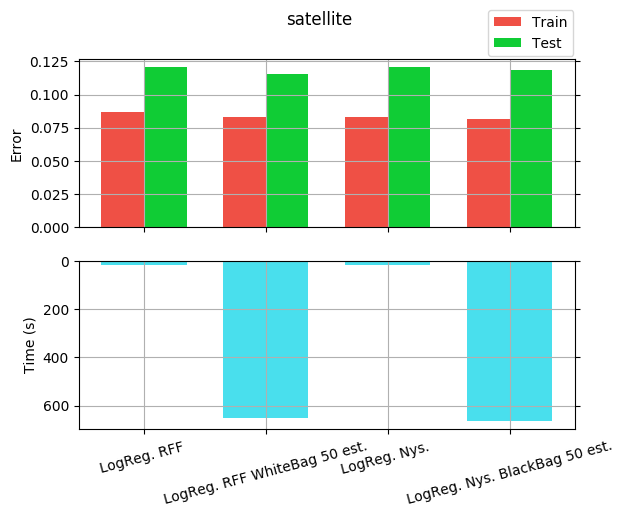
\includegraphics[width=\imgscale\linewidth]{Figures/\filePrefix/satellite}
    \caption{Exp 2.4 with \Nys\ with Satellite. Error is decreased by 7\% approx.}
    \label{fig:\undPrefix_satellite}
  \end{subfigure}
\end{figure}


\begin{figure}[H]
  \centering
  \renewcommand{\filePrefix}{\undPrefix/rff}
  \begin{subfigure}[t]{0.5\linewidth}
    \centering\captionsetup{width=.8\linewidth}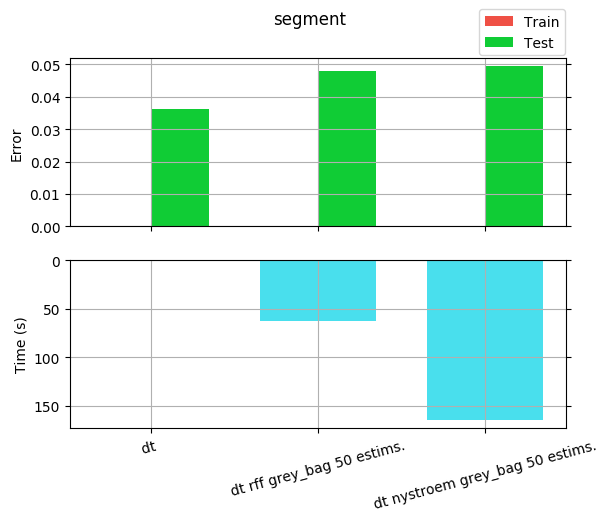
\includegraphics[width=\imgscale\linewidth]{Figures/\filePrefix/segment}
    \caption{Exp 2.4 with Random Fourier Feautures with Segment. Error is decreased by 2\% approx.}
    \label{fig:\undPrefix_segment}
  \end{subfigure}%
  \renewcommand{\filePrefix}{\undPrefix/nys}%
  \begin{subfigure}[t]{0.5\linewidth}
    \centering\captionsetup{width=.8\linewidth}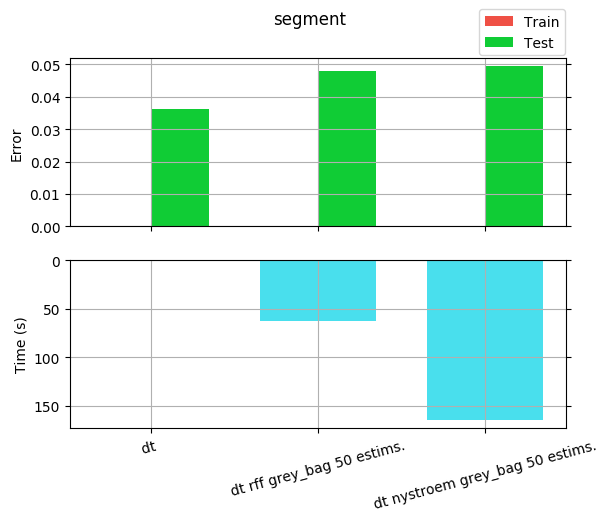
\includegraphics[width=\imgscale\linewidth]{Figures/\filePrefix/segment}
    \caption{Exp 2.4 with \Nys\ with Segment. Error is decreased by 2\% approx.}
    \label{fig:\undPrefix_segment}
  \end{subfigure}%
\end{figure}


\begin{figure}[H]
  \centering
  \renewcommand{\filePrefix}{\undPrefix/rff}
  \begin{subfigure}[t]{0.5\linewidth}
    \centering\captionsetup{width=.8\linewidth}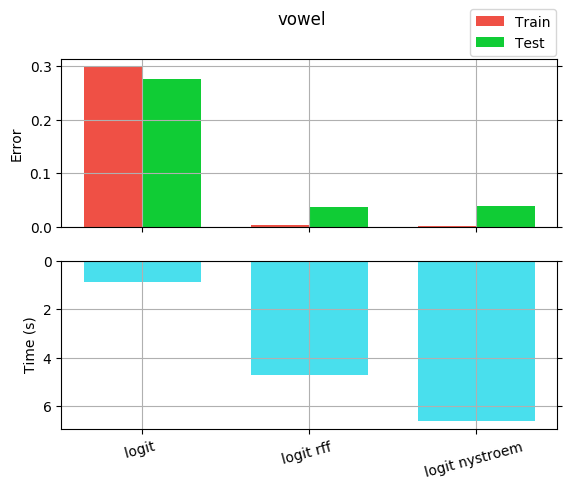
\includegraphics[width=\imgscale\linewidth]{Figures/\filePrefix/vowel}
    \caption{Exp 2.4 with Random Fourier Feautures with Vowel. Error is decreased by 38\% approx.}
    \label{fig:\undPrefix_vowel}
  \end{subfigure}%
  \renewcommand{\filePrefix}{\undPrefix/nys}%
  \begin{subfigure}[t]{0.5\linewidth}
    \centering\captionsetup{width=.8\linewidth}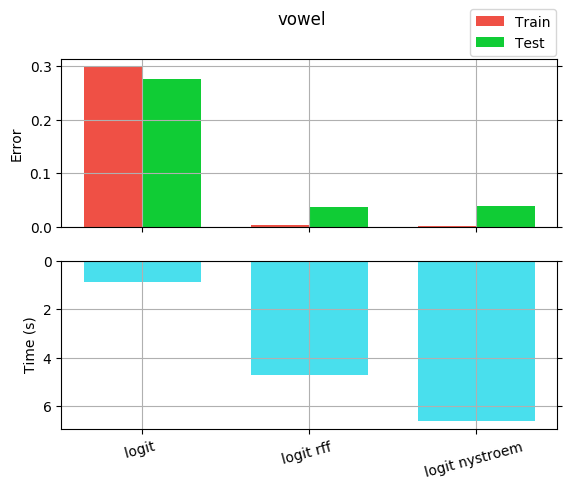
\includegraphics[width=\imgscale\linewidth]{Figures/\filePrefix/vowel}
    \caption{Exp 2.4 with \Nys\ with Vowel. Error is decreased by 38\% approx.}
    \label{fig:\undPrefix_vowel}
  \end{subfigure}
\end{figure}

%%%%%%%%%%%%%%%%%%%%%%%%%%%%%%%%%%%%%%%%%%%%%%
%%%%%%%%%%%%%%%%%%%%%%%%%%%%%%%%%%%%%%%%%%%%%%
%%%%%%%%%%%%%%%%%%%%%%%%%%%%%%%%%%%%%%%%%%%%%%
%% Termina lo nuevo
%%%%%%%%%%%%%%%%%%%%%%%%%%%%%%%%%%%%%%%%%%%%%%
%%%%%%%%%%%%%%%%%%%%%%%%%%%%%%%%%%%%%%%%%%%%%%
%%%%%%%%%%%%%%%%%%%%%%%%%%%%%%%%%%%%%%%%%%%%%%



% \begin{figure}[H]
%   \centering
%   \begin{subfigure}[t]{0.5\linewidth}
%     \centering\captionsetup{width=.8\linewidth}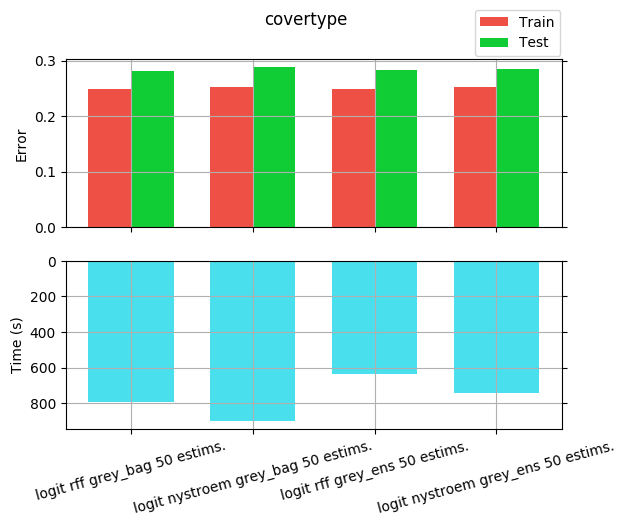
\includegraphics[width=\imgscale\linewidth]{Figures/\filePrefix/covertype}
%     \caption{Exp 2.4 with Random Fourier Feautures with Covertype. Error is decreased by 15\% approx.}
%     \label{fig:\undPrefix_covertype}
%   \end{subfigure}%
%   \begin{subfigure}[t]{0.5\linewidth}
%     \centering\captionsetup{width=.8\linewidth}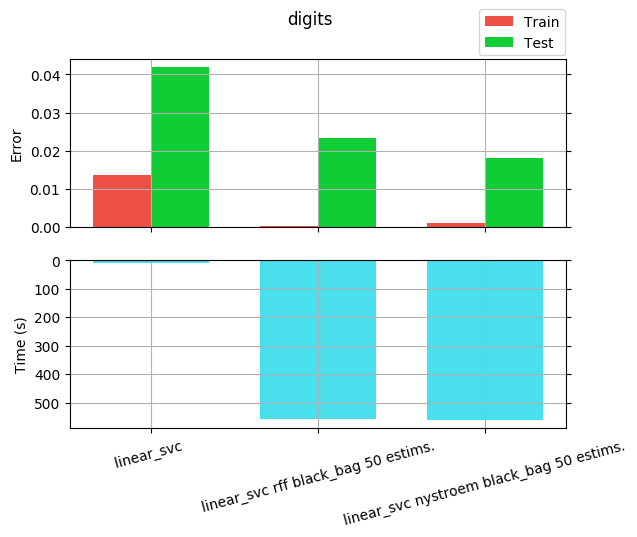
\includegraphics[width=\imgscale\linewidth]{Figures/\filePrefix/digits}
%     \caption{Exp 2.4 with Random Fourier Feautures with Digits. Error is decreased by 2\% approx.}
%     \label{fig:\undPrefix_digits}
%   \end{subfigure}
% \end{figure}
%
%
% \begin{figure}[H]
%   \centering
%   \begin{subfigure}[t]{0.5\linewidth}
%     \centering\captionsetup{width=.8\linewidth}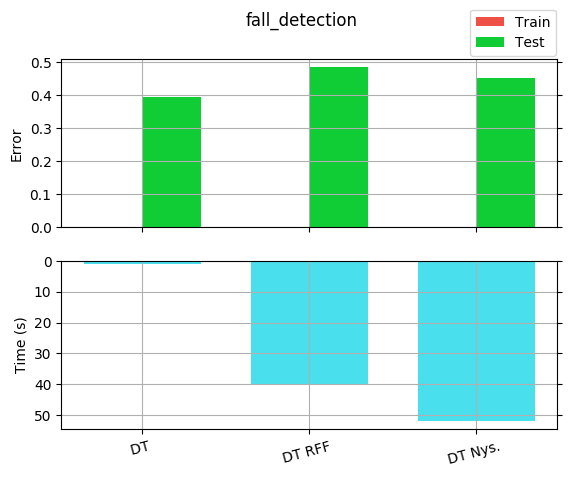
\includegraphics[width=\imgscale\linewidth]{Figures/\filePrefix/fall_detection}
%     \caption{Exp 2.4 with Random Fourier Feautures with Fall Detection. Error is decreased by 2\% approx.}
%     \label{fig:\undPrefix_fall_detection}
%   \end{subfigure}%
%   \begin{subfigure}[t]{0.5\linewidth}
%     \centering\captionsetup{width=.8\linewidth}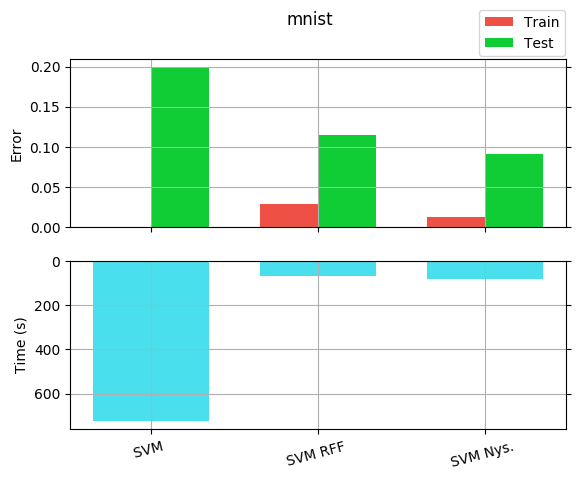
\includegraphics[width=\imgscale\linewidth]{Figures/\filePrefix/mnist}
%     \caption{Exp 2.4 with Random Fourier Feautures with MNIST. Error is decreased by 10\% approx.}
%     \label{fig:\undPrefix_mnist}
%   \end{subfigure}
% \end{figure}
%
%
% \begin{figure}[H]
%   \centering
%   \begin{subfigure}[t]{0.5\linewidth}
%     \centering\captionsetup{width=.8\linewidth}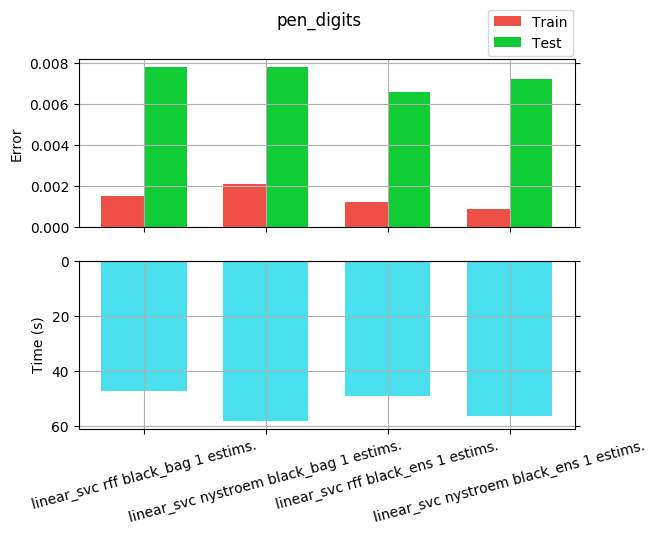
\includegraphics[width=\imgscale\linewidth]{Figures/\filePrefix/pen_digits}
%     \caption{Exp 2.4 with Random Fourier Feautures with Pen Digits. Error is decreased by 5\% approx.}
%     \label{fig:\undPrefix_pen_digits}
%   \end{subfigure}%
%   \begin{subfigure}[t]{0.5\linewidth}
%     \centering\captionsetup{width=.8\linewidth}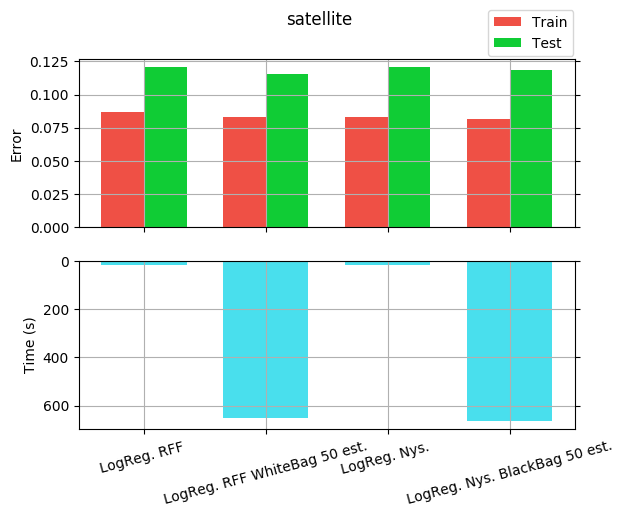
\includegraphics[width=\imgscale\linewidth]{Figures/\filePrefix/satellite}
%     \caption{Exp 2.4 with Random Fourier Feautures with Satellite. Error is decreased by 7\% approx.}
%     \label{fig:\undPrefix_satellite}
%   \end{subfigure}
% \end{figure}
%
% \begin{figure}[H]
%   \centering
%   \begin{subfigure}[t]{0.5\linewidth}
%     \centering\captionsetup{width=.8\linewidth}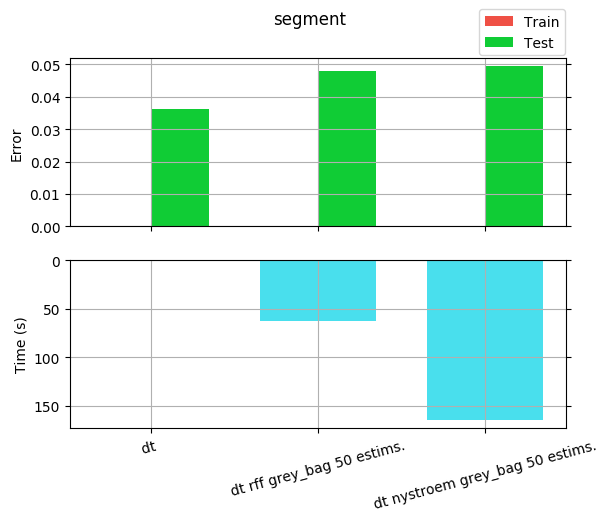
\includegraphics[width=\imgscale\linewidth]{Figures/\filePrefix/segment}
%     \caption{Exp 2.4 with Random Fourier Feautures with Segment. Error is decreased by 2\% approx.}
%     \label{fig:\undPrefix_segment}
%   \end{subfigure}%
%   \begin{subfigure}[t]{0.5\linewidth}
%     \centering\captionsetup{width=.8\linewidth}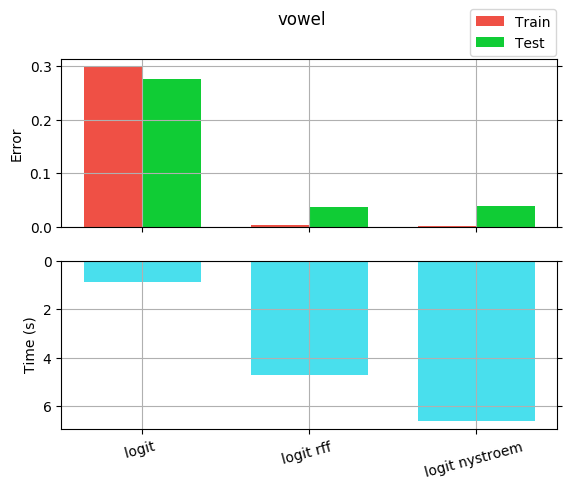
\includegraphics[width=\imgscale\linewidth]{Figures/\filePrefix/vowel}
%     \caption{Exp 2.4 with Random Fourier Feautures with Vowel. Error is decreased by 38\% approx.}
%     \label{fig:\undPrefix_vowel}
%   \end{subfigure}
% \end{figure}
%
% %%%%%%%%%%%%%%%%%%%%%%%%%%%%%%
%
% \renewcommand{\filePrefix}{\undPrefix/nys}
% \begin{figure}[H]
%   \centering
%   \begin{subfigure}[t]{0.5\linewidth}
%     \centering\captionsetup{width=.8\linewidth}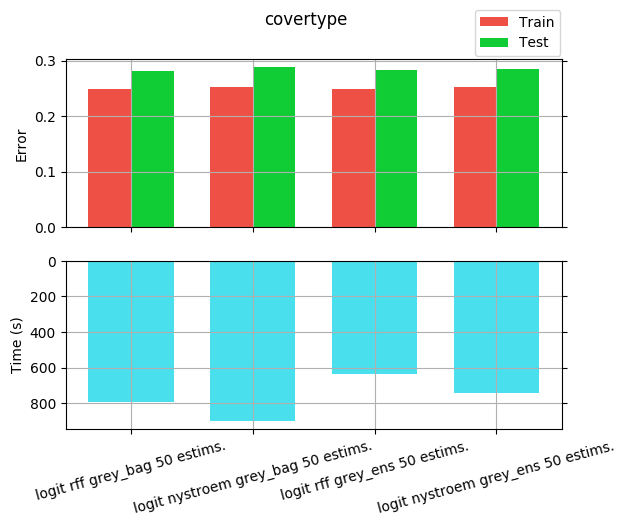
\includegraphics[width=\imgscale\linewidth]{Figures/\filePrefix/covertype}
%     \caption{Exp 2.4 with \Nys\ with Covertype. Error is decreased by 15\% approx.}
%     \label{fig:\undPrefix_covertype}
%   \end{subfigure}%
%   \begin{subfigure}[t]{0.5\linewidth}
%     \centering\captionsetup{width=.8\linewidth}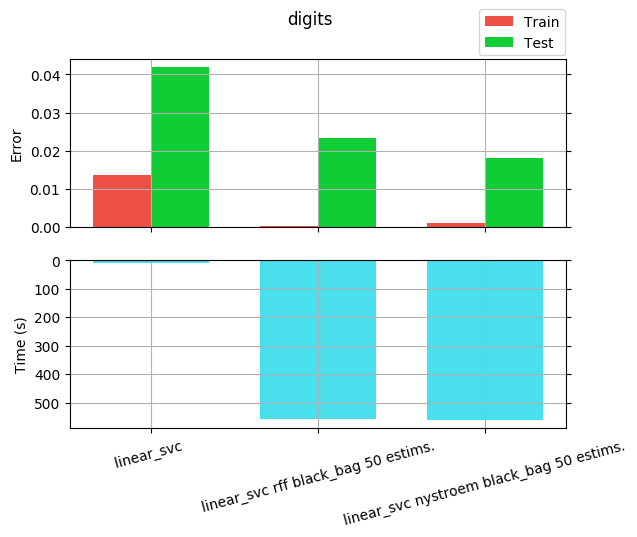
\includegraphics[width=\imgscale\linewidth]{Figures/\filePrefix/digits}
%     \caption{Exp 2.4 with \Nys\ with Digits. Error is decreased by 2\% approx.}
%     \label{fig:\undPrefix_digits}
%   \end{subfigure}
% \end{figure}
%
%
% \begin{figure}[H]
%   \centering
%   \begin{subfigure}[t]{0.5\linewidth}
%     \centering\captionsetup{width=.8\linewidth}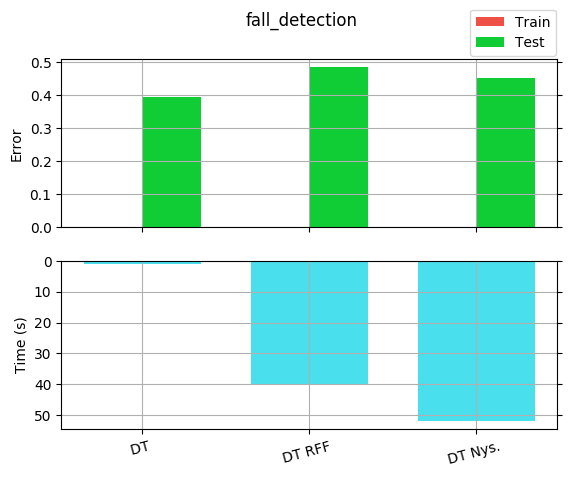
\includegraphics[width=\imgscale\linewidth]{Figures/\filePrefix/fall_detection}
%     \caption{Exp 2.4 with \Nys\ with Fall Detection. Error is decreased by 2\% approx.}
%     \label{fig:\undPrefix_fall_detection}
%   \end{subfigure}%
%   \begin{subfigure}[t]{0.5\linewidth}
%     \centering\captionsetup{width=.8\linewidth}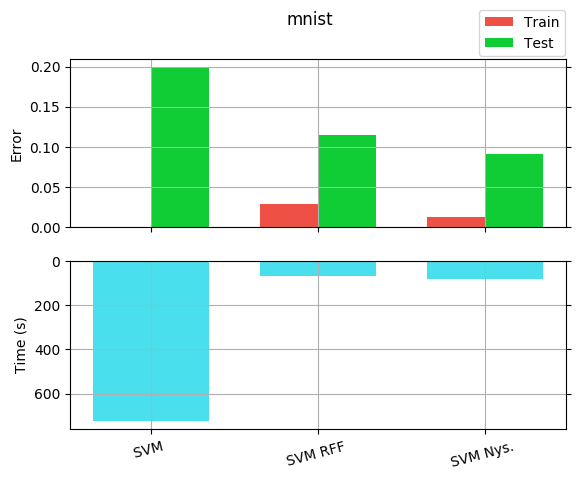
\includegraphics[width=\imgscale\linewidth]{Figures/\filePrefix/mnist}
%     \caption{Exp 2.4 with \Nys with MNIST. Error is decreased by 10\% approx.}
%     \label{fig:\undPrefix_mnist}
%   \end{subfigure}
% \end{figure}
%
%
% \begin{figure}[H]
%   \centering
%   \begin{subfigure}[t]{0.5\linewidth}
%     \centering\captionsetup{width=.8\linewidth}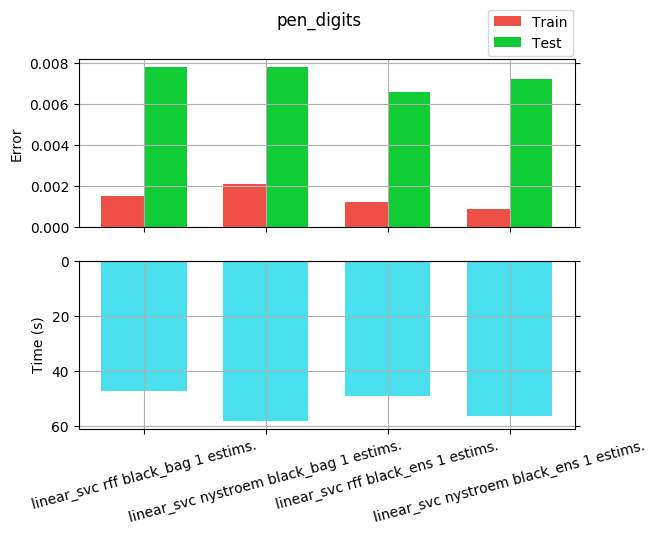
\includegraphics[width=\imgscale\linewidth]{Figures/\filePrefix/pen_digits}
%     \caption{Exp 2.4 with \Nys\ with Pen Digits. Error is decreased by 5\% approx.}
%     \label{fig:\undPrefix_pen_digits}
%   \end{subfigure}%
%   \begin{subfigure}[t]{0.5\linewidth}
%     \centering\captionsetup{width=.8\linewidth}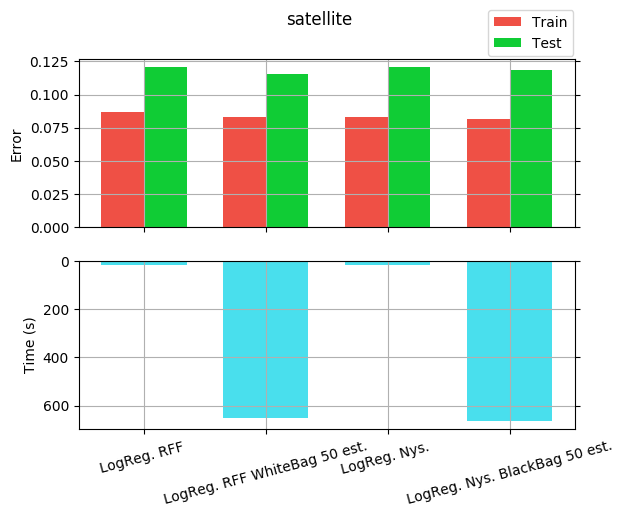
\includegraphics[width=\imgscale\linewidth]{Figures/\filePrefix/satellite}
%     \caption{Exp 2.4 with \Nys\ with Satellite. Error is decreased by 7\% approx.}
%     \label{fig:\undPrefix_satellite}
%   \end{subfigure}
% \end{figure}
%
% \begin{figure}[H]
%   \centering
%   \begin{subfigure}[t]{0.5\linewidth}
%     \centering\captionsetup{width=.8\linewidth}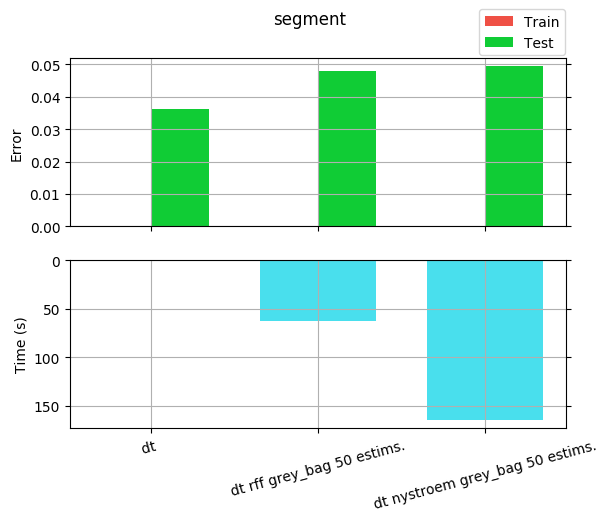
\includegraphics[width=\imgscale\linewidth]{Figures/\filePrefix/segment}
%     \caption{Exp 2.4 with \Nys\ with Segment. Error is decreased by 2\% approx.}
%     \label{fig:\undPrefix_segment}
%   \end{subfigure}%
%   \begin{subfigure}[t]{0.5\linewidth}
%     \centering\captionsetup{width=.8\linewidth}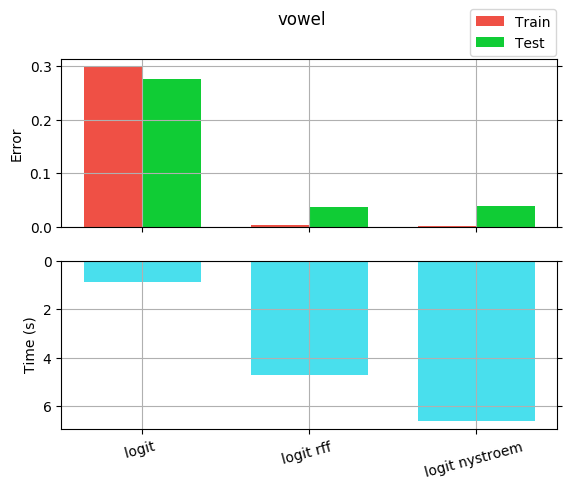
\includegraphics[width=\imgscale\linewidth]{Figures/\filePrefix/vowel}
%     \caption{Exp 2.4 with \Nys\ with Vowel. Error is decreased by 38\% approx.}
%     \label{fig:\undPrefix_vowel}
%   \end{subfigure}
% \end{figure}


%%%%%%%%%%%%%%%

{\LARGE Comparison of Single Model and Ensemble both using a random mapping}

\renewcommand{\filePrefix}{\undPrefix/aux}
\begin{figure}[H]
  \centering
  \begin{subfigure}[t]{0.5\linewidth}
    \centering\captionsetup{width=.8\linewidth}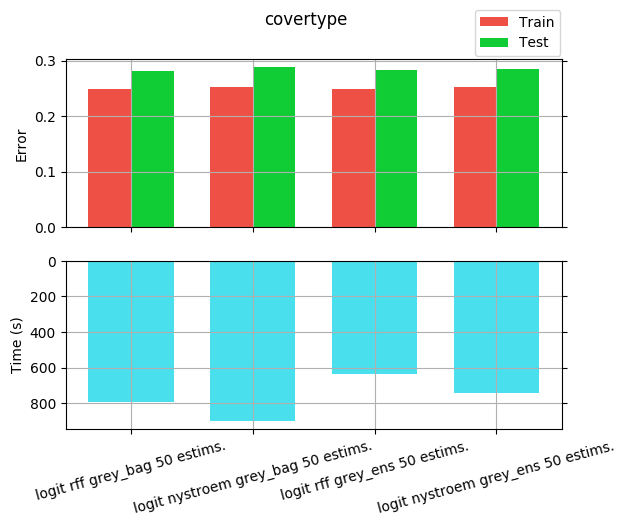
\includegraphics[width=\imgscale\linewidth]{Figures/\filePrefix/covertype}
    \caption{Support Vector Machine with random mapping. A single model vs. an Ensemble. There is not big difference with Covertype.}
    % \label{fig:\undPrefix_covertype}
    \label{2_4:aux}
  \end{subfigure}%
  \begin{subfigure}[t]{0.5\linewidth}
    \centering\captionsetup{width=.8\linewidth}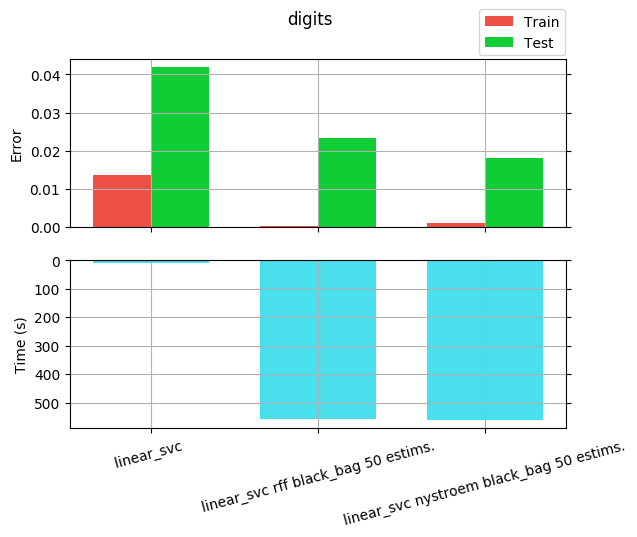
\includegraphics[width=\imgscale\linewidth]{Figures/\filePrefix/digits}
    \caption{Support Vector Machine with random mapping. A single model vs. an Ensemble. There is not big difference with Digits.}
    \label{fig:\undPrefix_digits}
  \end{subfigure}
\end{figure}


\begin{figure}[H]
  \centering
  \begin{subfigure}[t]{0.5\linewidth}
    \centering\captionsetup{width=.8\linewidth}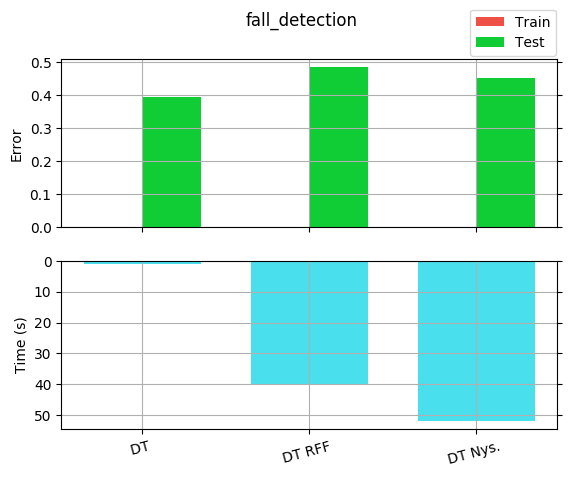
\includegraphics[width=\imgscale\linewidth]{Figures/\filePrefix/fall_detection}
    \caption{Support Vector Machine with random mapping. A single model vs. an Ensemble. There is not big difference with Fall Detection.}
    \label{fig:\undPrefix_fall_detection}
  \end{subfigure}%
  \begin{subfigure}[t]{0.5\linewidth}
    \centering\captionsetup{width=.8\linewidth}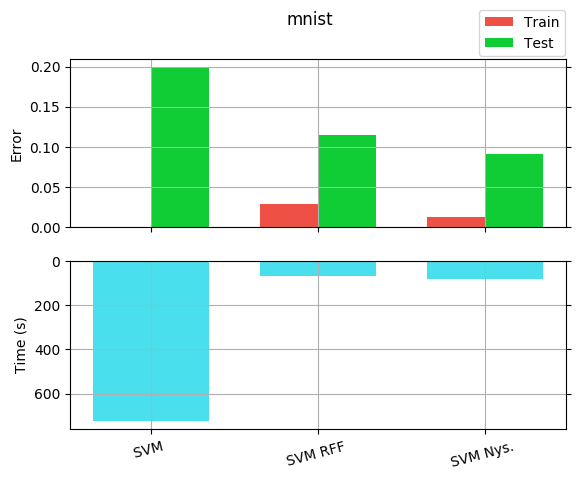
\includegraphics[width=\imgscale\linewidth]{Figures/\filePrefix/mnist}
    \caption{Support Vector Machine with random mapping. A single model vs. an Ensemble. There is not big difference with MNIST.}
    \label{fig:\undPrefix_mnist}
  \end{subfigure}
\end{figure}


\begin{figure}[H]
  \centering
  \begin{subfigure}[t]{0.5\linewidth}
    \centering\captionsetup{width=.8\linewidth}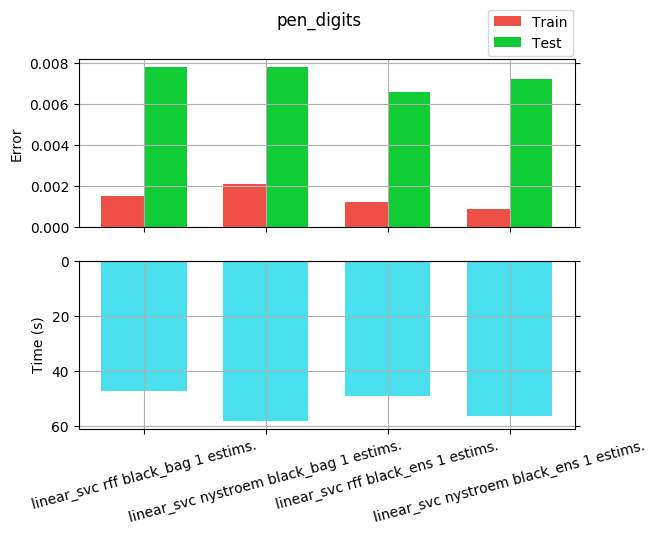
\includegraphics[width=\imgscale\linewidth]{Figures/\filePrefix/pen_digits}
    \caption{Support Vector Machine with random mapping. A single model vs. an Ensemble. There is not big difference with Pen Digits.}
    \label{fig:\undPrefix_pen_digits}
  \end{subfigure}%
  \begin{subfigure}[t]{0.5\linewidth}
    \centering\captionsetup{width=.8\linewidth}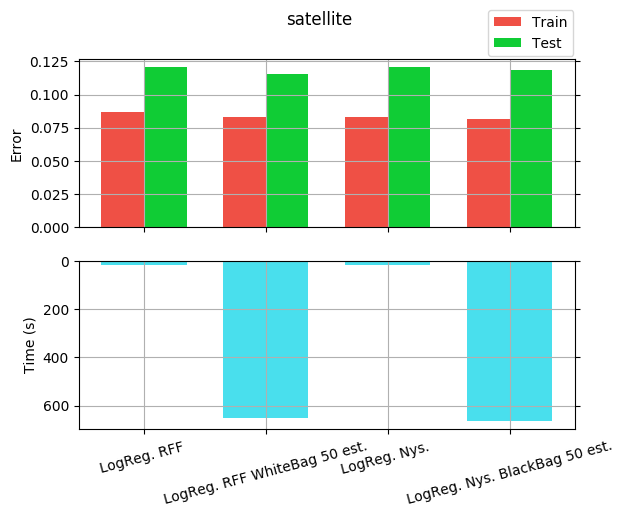
\includegraphics[width=\imgscale\linewidth]{Figures/\filePrefix/satellite}
    \caption{Support Vector Machine with random mapping. A single model vs. an Ensemble. There is not big difference with Satellite.}
    \label{fig:\undPrefix_satellite}
  \end{subfigure}
\end{figure}

\begin{figure}[H]
  \centering
  \begin{subfigure}[t]{0.5\linewidth}
    \centering\captionsetup{width=.8\linewidth}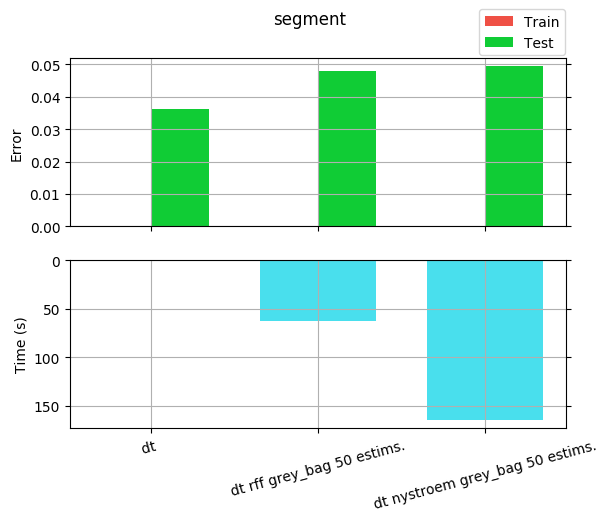
\includegraphics[width=\imgscale\linewidth]{Figures/\filePrefix/segment}
    \caption{Support Vector Machine with random mapping. A single model vs. an Ensemble. There is not big difference with Segment.}
    \label{fig:\undPrefix_segment}
  \end{subfigure}%
  \begin{subfigure}[t]{0.5\linewidth}
    \centering\captionsetup{width=.8\linewidth}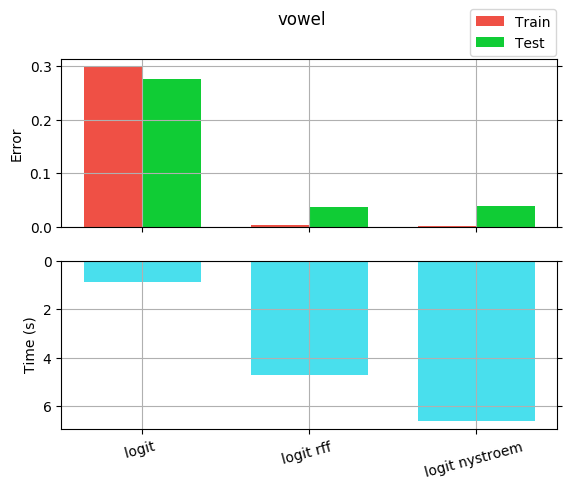
\includegraphics[width=\imgscale\linewidth]{Figures/\filePrefix/vowel}
    \caption{Support Vector Machine with random mapping. A single model vs. an Ensemble. There is not big difference with Vowel.}
    \label{fig:\undPrefix_vowel}
  \end{subfigure}
\end{figure}


\let\major\undefined
\let\minor\undefined

\let\undPrefix\undefined
\let\dotPrefix\undefined
\let\scoPrefix\undefined

\let\filePrefix\undefined
